\documentclass[a4paper,10pt]{report}
\usepackage[utf8x]{inputenc}
\usepackage[french]{babel}
\usepackage[T1]{fontenc}
\usepackage{latexsym}
\usepackage{algorithm,algorithmic}
\usepackage{graphicx}
\usepackage{amssymb, amsmath}

%%% francisation des algorithmes
\renewcommand{\algorithmicrequire} {\textbf{\textsc{Entrées:}}}
\renewcommand{\algorithmicensure}  {\textbf{\textsc{Sorties:}}}
\renewcommand{\algorithmicwhile}   {\textbf{tantque}}
\renewcommand{\algorithmicdo}      {\textbf{faire}}
\renewcommand{\algorithmicendwhile}{\textbf{fin tantque}}
\renewcommand{\algorithmicend}     {\textbf{fin}}
\renewcommand{\algorithmicif}      {\textbf{si}}
\renewcommand{\algorithmicendif}   {\textbf{finsi}}
\renewcommand{\algorithmicelse}    {\textbf{sinon}}
\renewcommand{\algorithmicthen}    {\textbf{alors}}
\renewcommand{\algorithmicfor}     {\textbf{pour}}
\renewcommand{\algorithmicforall}  {\textbf{pour tout}}
\renewcommand{\algorithmicdo}      {\textbf{faire}}
\renewcommand{\algorithmicendfor}  {\textbf{fin pour}}
\renewcommand{\algorithmicloop}    {\textbf{boucler}}
\renewcommand{\algorithmicendloop} {\textbf{fin boucle}}
\renewcommand{\algorithmicrepeat}  {\textbf{répéter}}
\renewcommand{\algorithmicuntil}   {\textbf{jusqu'à}}

\newcommand{\Fp}{\mathbb{F}_p}
\newcommand{\Pp}{\mathbb{P}_1(\Fp)}
\newcommand{\article}{\textit{On the correct use of the negation map in the Pollard rho method}}

% Title Page
\title{Algorithme rho de pollard}
\author{TAFFOREAU Nicolas}


% -----------------------------------------
% organisation a revoir 
% -----------------------------------------

\begin{document}
\maketitle
\tableofcontents
\chapter{Introduction}
Dans une première partie je montrerai de manière expérimenatale la complexité de l'algorithme rho de pollard. Dans une seconde partie j'introduirai une première amelioration par un facteur constant de cette methode, en utilisant 
une marche aléatoire différente de celle initiale de pollard. Ma troisième partie constitue une parallélisation de la methode de pollard. Ma partie finale parlera de la methode de 'negation map' introduit dans 
'\textit{On the correct use of the negation map in the Pollard rho method}' qui permet de reduire le temps de la methode par une facteur $\sqrt{2}$.
\section{Rappel sur les courbes elliptique}
% 2 pages

%
Soit $\mathcal{E}:(YZ^2+a_1XYZ+a_3YZ^2)-(X^3+a_2X^2Z+a_4XZ^2+a_6Z^3)$ avec $(a_1,a_2,a_3,a_4,a_6) \in K $.\\


La forme courte de Weierstass est définie par : $a_1=a_2=a_3=0 $. La courbe a donc l'équation suivante :
$$ \mathcal{E} : Y^2Z=X^3+aXZ^2+bZ^3 $$
$$ -4a^3+27b^2 \neq 0 $$

% 
   Soit un corps $\Fp$ ($p > 3$ premier), et soit $a, b \in \Fp$
tels que $4 a^3 + 27 b^2 \ne 0$.
La courbe elliptique $E/\Fp: Y^2 = X^3 + aX + b$ est définie par l'ensemble
des points $(x:y:z)\in \Pp$ tel que soit satifaite l'équation 
$$ z y^2 = x^3 + a x z^2 + b z^3.$$

  Si z = 0 alors x = 0 et donc on obtient $(0,k,0)$ qui est un élément inversible donc peut être réduit à $(0,1,0)$, ce point scpécifique est appelé le point à l'infini.

  L'ensemble de ces points forment un groupe abélien avec comme zero, le point à l'infini et possède un loi de groupe.
  Soit P, $Q \in F$, $ P = (x_1,y_1)$, $Q = (x_2,y_2)$ alors $P+Q = (x_3,y_3)$ tel que 
    \begin{center}
      $x_3 = \mu^2 -x_1 - x_2$, $y_3 = \mu(x_1-x_3)$ \\
$ \mu =  \left\{
    \begin{array}{ll}
        \displaystyle \frac{y_2 - y_1}{x_2 - x_1} & $si $P \ne Q  \\
        \\      
        \displaystyle \frac{3*x_1^2 + a}{2*y_1} & $si $P = Q
    \end{array}
\right.$ \\
\end{center}

Une propriété importante sur les courbes elliptiques est le calcule de l'inverse d'un point pour la loi d'addition sur Fp. Si $P = (x_1,y_1)$ alors $-P = (x_1,-y_1)$.

\section{Algorithme rho de Pollard}

Dans une suite d'éléments $S(n)$, un cycle est un ensemble d'éléments fini tel que ces éléments réaparaisse de façon périodique dans la suite $S(n)$, on peut avoir avant un cycle un pré-cycle de longueur finie.
Si $\lambda$ est la longueur du pré-cycle et $\mu$ la longueur du cycle on aura pour tout $i > 0$, $S_{\lambda+i} = S_{\lambda+\mu+i}$ .

Une marche aléatoire discrète est une suite où 

\subsection{Dans un groupe du type Fp}

Dans un groupe du type Fp, Pollard a choisit comme marche aléatoire un fonction qui ne tient compte que de l'élément précédent.\\

\begin{description}
\item{Marche aléatoire}\\
{
$ f(x) = x*P$ si $x \in [0;p/3[$\\
$ f(x) = x*x$ si $x \in [p/3;2p/3[$\\
$ f(x) = x*Q$ si $x \in [2p/3;p[$\\
}
\end{description}

En utilisant cette marche aléatoire il en a deduit un algorithme en se basant sur l'algorithme de floyd pour trouver rapidement la longueur d'un cycle.

Ici P est un generateur du groupe et Q est l'élément dont on veut connaitre le logarithme en base P.
 
{
 \begin{algorithm}
 \caption{rho pollard}
 \begin{algorithmic}
  \REQUIRE n,P,Q
  \ENSURE x tel que Q = $P^x$ mod n
  \STATE $[W1,a,b] \leftarrow$ combinaision aleatoire de $P$ et $Q$
    \STATE $[W2,a',b'] \leftarrow$  marche aléatoire à partir de $W1$
	\STATE ($W2 = P^{a'} + Q^{b'}$)
    \WHILE{$ W1 \ne W2$}
      \STATE $[W1,a,b] \leftarrow$ marche aléatoire à partir de $W1$
      \STATE $[W2,a',b'] \leftarrow$ marche aléatoire à partir de $W2$
      \STATE $[W2,a',b'] \leftarrow$ marche aléatoire à partir de $W2$
    \ENDWHILE
  \IF{ $b-b' = 0$ $modulo$ $n$}
    \STATE echec pour trouver le logarithme discret
  \ELSE
    \STATE $ x = \frac{a'-a}{b-b'}$ $modulo$ $n$
  \ENDIF
 
 \end{algorithmic}
 \end{algorithm}
 }


L'algorithme rho de pollard est identique sur les courbes elliptiques sauf que l'on se place dans un cas plus générale,
seul la marche aléatoire change. On applique des additions et de scalaires sur la courbe elliptique au lieu de la multiplication modulaire et du carré modulaire.

Le nom de cette algorithme est dû à la forme que prend la suite aléatoire, on a d'abord un pré-cycle puis le cycle.

\begin{center}
 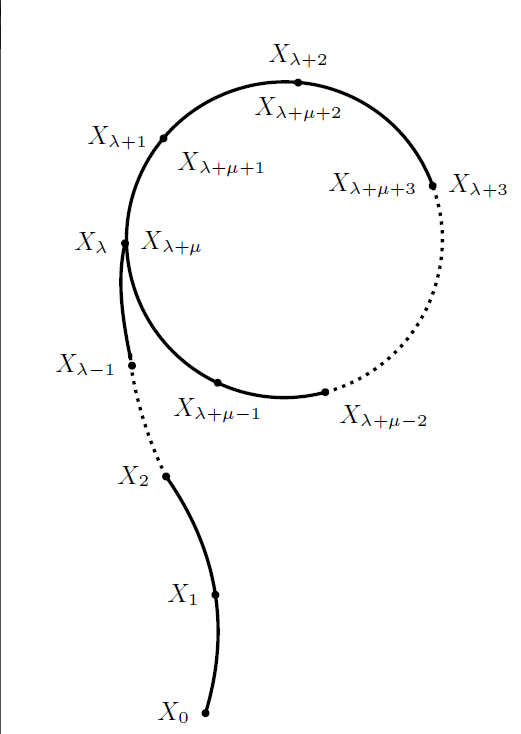
\includegraphics[width=4cm]{dessin_rho_pollard_bon.png}
\end{center}

\subsection{Paradoxe des Anniversaires}
L'algorithme rho de pollard est basé sur le paradoxe des anniversaires.

 Dans un groupe fini si on prend des éléments de façon aléatoire,
il faut en moyenne tirer $\sqrt{n}$ éléments pour obtenir un élément que l'on à déjà tiré, ou n est le nombre d'élément de notre ensemble.

La formule générale pour obtenir une probabilité d'intersection ($I(n)$) est 1-$p(n)$ où $p(n)$ est la probabilité d'avoir aucune intersetion sur n tirages avec remise dans un groupe de $m$ éléments
\begin{center}
    $p(n) = \frac{m!}{(m - n)!}*\frac{1}{m^n}$
    $I(n) = 1 - \frac{m!}{(m - n)!}*\frac{1}{m^n}$
\end{center}


\chapter{Comlpexité de l'algorithme rho de pollard}

L'algorithme rho de pollard est estimé, d'après le papier de Stephen D. Miller et Ramarathnam Venkatesan, \textit{Spectral Analysis of Pollard Rho Collisions} en $O(\sqrt{n}(\log{n})^3)$. 
Quand n temps vers l'infini le logarithme est négligeable par rapport à la racine de n. On peut donc approximé cette complexité en $O(\sqrt{n})$.

Pour montrer que l'algorithme est bien dans une complexité s'approchant de la racine de n, j'ai effectué des tests de résolutions du logarithme discret avec la methode initiale
de Pollard. La marche aléatoire que j'ai pris est définie par : \\

\begin{description}
\item{Marche aléatoire}\\
  $ f(W) = W \oplus P$ si $x = 0$ $modulo$ $3$ \\
  $ f(W) = 2*W$ si $x = 1$ $modulo$ $3$ \\
  $ f(W) = W \oplus Q$ si $x = 2$  $modulo$ $3$ \\
  $ W = [x,y] $ \\
\end{description}

Dans '\article', Bernstein, Lange et Schwabe prenne des courbes elliptiques avec $a = -3$, en faisant des tests sur d'autre courbe avec un $a$a tiré aléatoirement j'obtient les même temps pour
retrouver le logarithmes discret. J'ai donc pour plus de simplicité garder le $a=-3$ dans mes tests généraux.
Pour ne pas avoir de problème d'inversement lors de la dernière étape de l'algorithme de pollard j'ai pris seulement des courbes avec une cardinalité première.

Ici le $\oplus$ est l'addition sur la courbe elliptique et le $2*W$ est l'oppération de doublement sur la courbe elliptique.

Pour obtenir des valeurs faciles pour faire une comparaison, il est plus simple de changer l'échelle et de regarder en echelle logarithmique.
( $\sqrt{n} = n^{\frac{1}{2}}$ )
 Si $n=2^x$ alors en échelle logarithimque (base 2) $\log{n} = x$ et $\log{\sqrt{n}} = \frac{x}{2}$

Donc si on fait une régression linéaire des différents valeurs trouvées, on devrait obtenir une droite avec un coefficient de $0,5$.

\newpage
$$f(x) = ax + b $$


\begin{verbatim}
degrees of freedom    (FIT_NDF)                        : 34
rms of residuals      (FIT_STDFIT) = sqrt(WSSR/ndf)    : 0.197332
variance of residuals (reduced chisquare) = WSSR/ndf   : 0.0389399

Final set of parameters            Asymptotic Standard Error
=======================            ==========================

a               = 0.48823          +/- 0.002987     (0.6118%)
b               = -5.24743         +/- 0.09242      (1.761%)
\end{verbatim}

On otient donc une valeur pour $a$ proche de $0,5$.\\

On peut donc grâce à cette régrssion linéaire prévoir le temps de calcule pour des logarithmes sur courbes elliptiques de plus grande cardinalité.

\begin{center}
 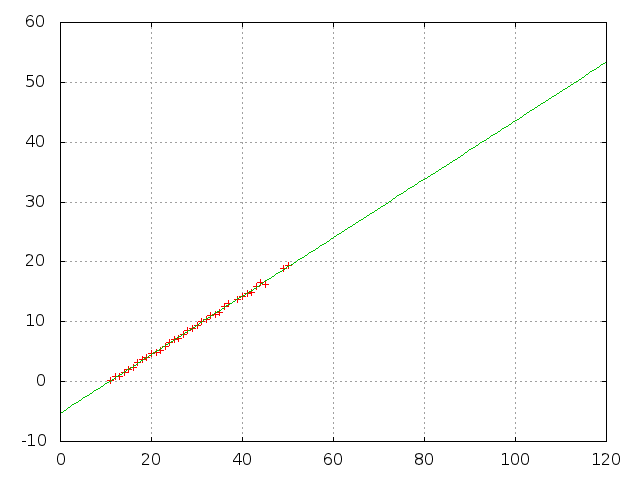
\includegraphics[width=13cm]{rho_normal.png}
 Temps d'execution (échelle logarithmique) de la methode rho de pollard en fonction du nombre de bit de la courbe.
\end{center}

Dans l'article \article, Bernstein prend l'exemple du logarithme discret sur courbe elliptique secp112r1 qui est un log discret sur 112 bits. En regardant la courbe on peut voir qu'il faudrait environs 25 millénaires 
($\exp{((\log{2})*49.5)}$) pour résoudre le logarithme discret.


\chapter{Marche aléatoire avec plusieurs groupes}

\section{Indice de}
Dans l'article de \textit{Bernstein}, il est fait référence au fait que \textit{Pollard} n'utilisait que trois groupes pour faire sa marche aléatoire, 
alors que Teske dans son papier \textit{On random walks for pollard's rho method}, nous dit qu'il est beaucoup plus efficase d'utiliser plus de groupe pour faire une marche aléatoire.
\newline

Dans son article \textit{Teske} introduit l'indice L :
\begin{center}
 $ L = \frac{\text{nombre d'iteration avant de trouver une collision}}{\sqrt(|G|)} $
\end{center}

Après plusieurs tests expérimetales la valeur que j'ai pour cette indice, en utlisant la méthode normale est environs $1,3$.\\

\section{Amélioration multi-groupe}

J'ai donc implémenté une fonction qui au lieu d'utiliser une marche aléatoire sur trois groupes en faisant soit $\oplus P$, $\oplus Q$, ou un doublement,
utilise r groupes. Cette marche ajoute donc à chaque menbre de la suite entrante un élément spécifique du groupe en fonction d'une propriété du menbre entrant. Ces différents éléments sont au préalable tiré aléatoirement
à partir d'une combinaison de $P$ et $Q$. Je fais donc une marche additive, pour chaque $W_i$ je lui ajoute un $R_j$ où j est un hash de i. On a donc la formule suivante : 
\begin{center}
$ W_{i+1} = W_{i} + R_{h(i)} $.
\end{center}

Chaque éléments $R_{h(i)}$ est de la forme $ [a_{h(i)}]P + [b_{h(i)}]Q$, où $a_{h(i)}$ et $b_{h(i)}$ sont des scalaires qui ont été tiré aléatoirement lors de l'initialisation du groupe.\\

la fonction  de hachage que je prend pour séparer les different élements dans les différent groupes est de prendre l'abscisse du point de la courbe elliptique modulo r.

\textit{Teske} après expérimentation trouve que pour la valeur $r >= 20$ ont atteint un bien meilleur ratio pour l'indice L.

En refaisant les tests j'obtient une zone de valeurs pour lesquel la valeur de L est petite. On peut dire que pour $ r > 18$ on obtient une faible valeur pour L et qu'elle ne change pas trop.
On remarque que pour la variation du temps en fonction du nombre de groupe, elle admet un pic minimun au alentour de la même valeur $18$. Le temps recommence à augmenter de manière linéaire
car on le temps de calcule des points pour créer les differents groupes qui n'est plus négligeable par rapport au reste de l'algorithme.
\begin{center}
  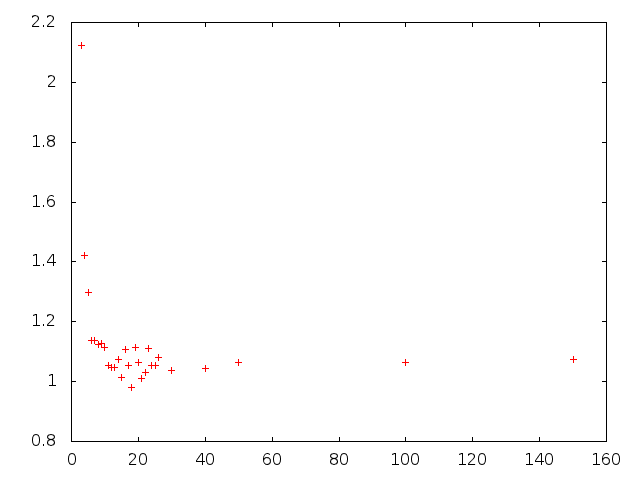
\includegraphics[width = 9cm]{variation_L.png}\\
  Variation de L en fonction du normbre de groupe\\
    pour la marche aléatoire.
\end{center}

\begin{center}
  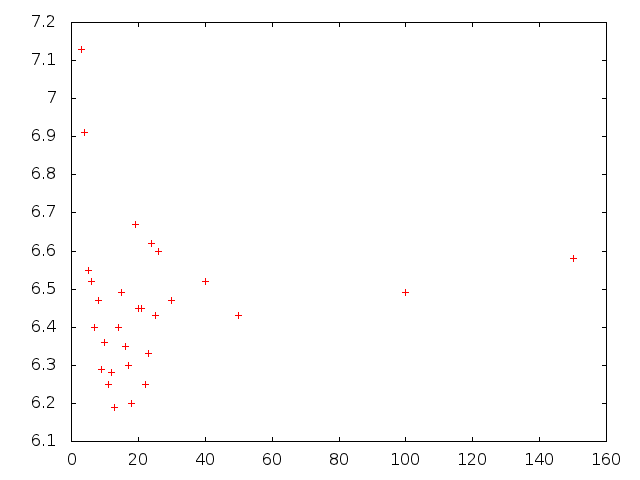
\includegraphics[width = 9cm]{variation_temps_en_fct_nbre_groupe.png}\\
  Variation du temps en fonction du normbre de groupe\\
    pour la marche aléatoire.
\end{center}

En refaisant une serie de tests avec cette première évaluation, j'obtient de nouveau temps inféreieur à la methode normale de Pollard.
\begin{center}
  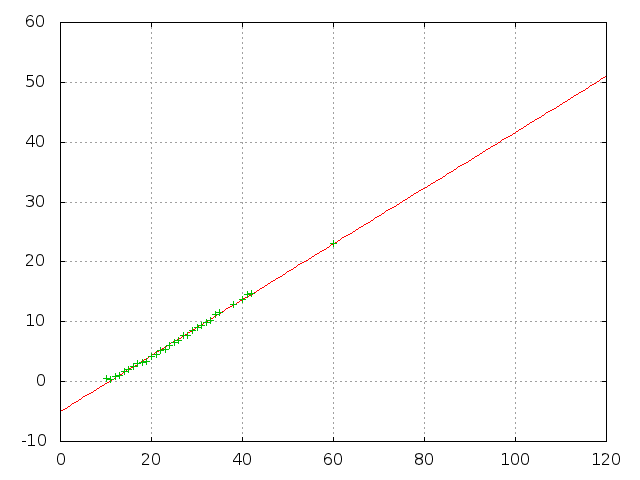
\includegraphics[width = 13cm]{rho_multi.png}
  Regresion linéaire de la methode rho avec\\
 une marche aléatoire avec 20 groupes
\end{center}

On obtient une regression linéaire avec un coefficient $a$ plus petit que la methode normale.

\begin{verbatim}
 degrees of freedom    (FIT_NDF)                        : 29
rms of residuals      (FIT_STDFIT) = sqrt(WSSR/ndf)    : 0.255346
variance of residuals (reduced chisquare) = WSSR/ndf   : 0.0652014

Final set of parameters            Asymptotic Standard Error
=======================            ==========================

c               = 0.466206         +/- 0.004165     (0.8935%)
d               = -4.979           +/- 0.1176       (2.362%)
\end{verbatim}


\newpage
On peut donc comparer les deux courbes et voir une légère différence.
\begin{center}
  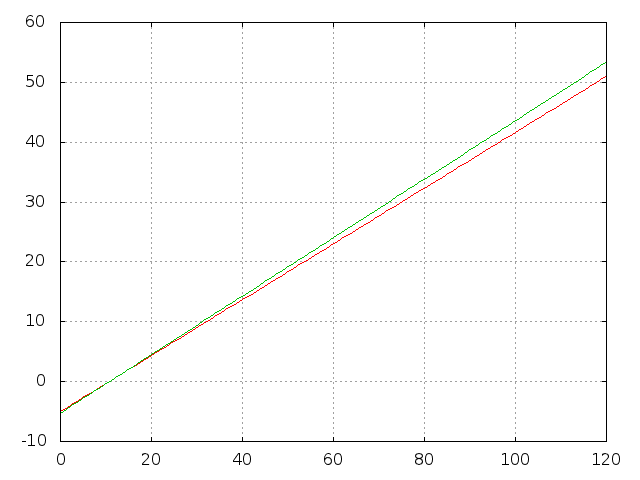
\includegraphics[width = 13cm]{compa_normal_multi.png}
   Comparaison entre le temps de l'algorithme normale\\
   et le temps de l'algorithme utilisant une marche aléatoire de 20 groupes.
\end{center}


Pour comparer toujours avec le logarithme sur une courbe elliptique d'un corps de $112$ bits,  on mettrait un peu plus de 5 millénaires ($\exp{((\log{2})*47.2)}$) pour résoudre le logarithme discret.

On a donc diviser le temps par un facteur 5.

\chapter{Parrallelisation de la méthode}

Pour pouvoir parraleliser le logarithme discret on a besoin de que de changer un peu le procedé de calcule. On n'a plus une unique boucle qui cherche directement le logarithme, mais plusieurs boucles qui cherche indépendament 
les une des autres des point de la courbes ayant une propriétés définie à l'avance et d'une boucle principale qui cherche les intercetions des points trouver par les autres boucle.

On a donc un serveur centrale qui s'occupe de faire la boucle principale en cherchant des collisions et plusieurs processeurs independants qui font une marche aléatoire pour trouver des points distingués de la courbe puis qui envoient
leurs points au serveur.

\section{Choix des points distingués}

Mon choix est de prendre des points dont la première variable (x) possède une certaine propriété tel que être congrue à un
 certain nombre pris aléatoirement. J'ai choisie de manière arbitraire que la coordonnée x devrait avoir ces n bits de poid 
faible égaux aux n bits de poid faible de $123456789$.

J'ai fait différents tests pour voir la proportion de points distingués dans une courbe elliptique en faisant soit varié la 
taille de la courbe elliptique, soit le nombre de bits pris.

\begin{center}
  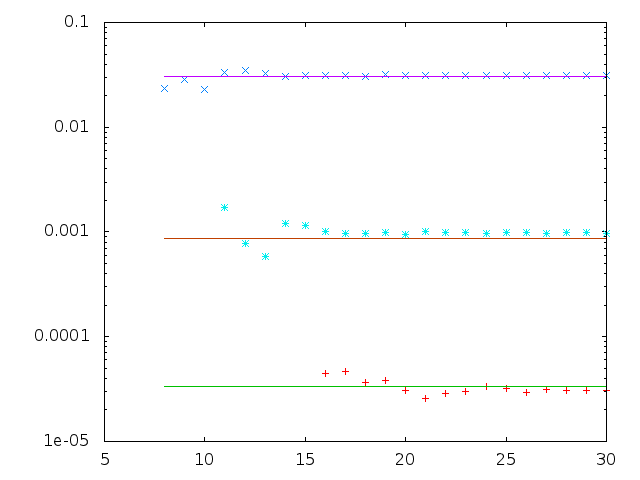
\includegraphics[width = 6.5cm]{courbe_pourcentage_different_point_distingue.png}\\
Proportion des points distingués en fonction \\
 de la taille de la courbe (échelle logarithmique).
\end{center}

 Avec ce premier graphique, on voit que la proportion de points distingués ne varie pas en fonction de la taille du groupe.\\

Maintenant regardons comment évolue cette proportion lorsqu'on change le nombre de bit observé.

\begin{verbatim}
# cardinalité courbe 20 bits
1 0.500522796 ~ 1/2^1 = 0.5
2 0.249615775 ~ 1/2^2 = 0.25
3 0.124589751 ~ 1/2^3 = 0.125
4 0.062905762 ~ 1/2^4 = 0.0625
5 0.031109468 ~ 1/2^5 = 0.03125
6 0.015635578 ~ 1/2^6 = 0.015625
7 0.007925448 ~ 1/2^7 = 0.0078125
8 0.003887007 ~ 1/2^8 = 0.00390625
9 0.001867395 ~ 1/2^9 = 0.001953125
10 0.00099737 ~ 1/2^10 = 0.000976562
11 0.00048597 ~ 1/2^11 = 0.000488281
12 0.00022821 ~ 1/2^12 = 0.000244140
13 0.00013557 ~ 1/2^13 = 0.000122070
14 0.00005802 ~ 1/2^14 = 0.000061035
15 0.00003040 ~ 1/2^15 = 0.000030517
16 0.00001806 ~ 1/2^16 = 0.000015258
17 0.00000262 ~ 1/2^17 = 0.000007629
18 0.00000380 ~ 1/2^18 = 0.000003814
19 0.00000259 ~ 1/2^19 = 0.000001907
\end{verbatim}

On remarque que les proportions sont de la forme $1/2^n$, elles diffèrent légèrement parfois car la cardinalité des courbes n'est pas
totalement $2^{20}$ mais est compris dans la borne de Hasse.

Ces résultats nous montrent que notre propriété est indépendante de la courbe.

\section{Amélioration programme parallèle}

\subsection{Amélioration en fonction du nombre de processus}

Le principe de parallelisation doit ralentir une méthode de recherche normale car on fait une double recherche au lieu d'utiliser
un algorithme de floyd. On va donc regarder à partir de combien, en moyenne, de processeur cette methode est équivalente à une methode normale.

On peut s'attendre à ce que l'évolution soit définie de façon simple car le serveur recherche de façon linéaire une collision quelque soit le nombre de prosséceur lui envoyant des données.
Donc on aura une collision après avoir trouvés environ la racine du nombre de points distingués de la courbe elliptique. Donc plus on a de processeur qui cherchent et envoient des 
points distingués au serveur plus rapidement on trouvera une collision, en supposant que le serveur n'a pas de problème a bouclé pour trouvé une collision. Pour éviter que le serveur n'ai trop de travail 
et soit ralenti, on doit choisir une propriété sur les point distingués qui permet d'avoir un nombre raisonnable de points.

Donc si nous avons un serveur qui ne prend qu'un temps plus petit par rapport au processeur qui doivent trouver des points, alors en augmentant le nombre de prosséceurs, le serveur recevra plus de points 
donc trouvera plus rapidement une collision. Par exemple si on a 20 processeurs alors si on utilise 21 processeurs on trouvera en théoriquement $21/20$ fois plus rapidement le logarithme discret que avec nos 20 processeurs.

\begin{center}
%  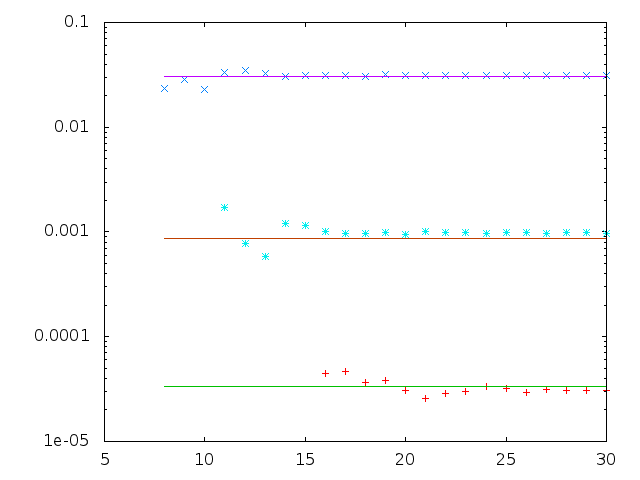
\includegraphics[width = 13cm]{courbe_pourcentage_different_point_distingue.png}\\
	Variation du temps en fonction du nombre\\
	de processus cherchant des points distingués.
\end{center}


\subsection{Ameliration par rapport à la méthode normale}

Donc avec un nombre assez élevés de processeur, on peut regarder la différence de temps entre la méthode normale de Pollard et la parallélisation.

\begin{center}
%  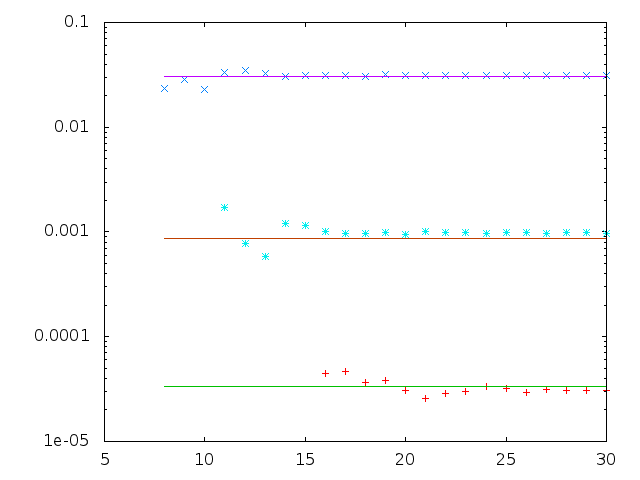
\includegraphics[width = 13cm]{courbe_pourcentage_different_point_distingue.png}\\
  Comparaison entre la méthode normale de pollard\\
 et une parallélisation de l'algorithme (avec XX processus).
\end{center}

Pour comparer avec les 

\section{Amélioration parallèle et mutlti-groupe}


\chapter{Negation map}

\section{methode general}

Soit E, une courbe elliptique sur $\Fp$ l'inverse de $P = (x,y,z)$, simplifié à $(x,y)$ est $-P = (x,-y)$. le but de cette méthode est de reduire le groupe de moitié,
donc de faire une recherche de logarithme discret dans un sousgroupe de E($\Fp$). On obtient donc une relation du type $\pm[a]P \pm[b]Q = \pm[a']P \pm[b']Q$. Il nous suffit donc de retrouver exactement 
la relation avec les bons signes pour retrouver le logarithme discret.\\

On va donc avoir un algorithme qui après la marche aléatoire regarde une propriété de notre nombre pour divisé la taille du groupe en deux. La propriété utilisée dans \article est de garder seulement le minimun du point ou son 
inverse de son inverse. D'autres propriétées peuvent être utilisée pour séparer le groupe en 2, elles sont tous basé sur l'utilisation du point et de son inverse seul el test varie.\\

On rencontre très rapidement un problème, l'apparision de cycle court de longueur $2$ qui empèche d'avoir une intersection dans note marche aléatoire.

La méthode décrite dans l'article \article, nous dis de garder en mémoire quelque points de la marche aléatoire, puis de faire un comparaison pour detecter si on entre dans un cycle
longueur 2, cette comparaison s'effectue entre le terme que l'on vient de calculer et celui qui était deux crant avant.
S'ils sont différents alors on continue la marche comme elle était, mais s'ils sont identiques alors le point suivant est $2*min(W_{-1},W_{-2})$ où le min est le minimun lexicographique et
la multiplication par 2 est l'oppération de doublement sur la courbe elliptique.



\chapter{bibliograpie}
Edlyn Teske, \textit{on a random walks for pollard's rho method}.

Daniel J. Bernstein, Tanja Lange, Peter Schwabe, \article.

John M.Pollard, \textit{monte carlo method for index computation mod p}.

Wikipedia.
\end{document}          
